
\documentclass{article}
\usepackage{amsmath,amssymb}
\usepackage[inline]{enumitem}
\usepackage{blindtext}
\usepackage{booktabs}
\usepackage{graphicx}
\usepackage{xcolor}
\usepackage[vmargin = 1.5in, top = 1in, bottom = 1.2in, letterpaper]{geometry}
\usepackage{listings}
\usepackage{courier}
\usepackage{multicol}
\usepackage{multirow}
\usepackage{bm}
\lstset{
basicstyle = \small\tt,
keywordstyle = \tt\color{blue},
commentstyle = \it\color[cmyk]{1,0,1,0},
stringstyle = \tt\color[RGB]{128,0,0},
%frame = single,
backgroundcolor = \color[RGB]{245,245,244},
breaklines,
extendedchars = false,
xleftmargin = 2em,
xrightmargin = 2em,
aboveskip = 1em,
tabsize = 4,
showspaces = false
}
\begin{document}
\setcounter{MaxMatrixCols}{20}

% \newfontfamily\courier{Courier New}


\title{STAT 510 Homework 9}
\author{Yifan Zhu}
\maketitle

\begin{enumerate}[leftmargin = 0 em, label = \arabic*., font = \bfseries]
	\item
	\begin{enumerate}
		\item \ 

		\begin{tabular}{l|rrr}
		\toprule
			& \multicolumn{3}{c}{geno}\\
			fert & 1 & 2 & 3\\
			\hline
			0 & 125 & 140 & 115\\
			50 & 141.25 & 156.25 & 141.25\\
			100 & 150 & 165 & 160 \\
			150 & 151.25 & 166.25 & 171.25\\
			\bottomrule
		\end{tabular}

		\item 
		Not true.
		\item 
		Not true.
		\item 
		Not true.
		\item 
		Geno Type 1:
		\[ E(y) = 125 + 0.4 f -0.0015 f^2\]
		Geno Type 2:
		\[ E(y) = 140 + 0.4 f - 0.0015 f^2\]
		Geno Type 3:
		\[ E(y) = 115 + 0.6 f - 0.0015 f^2\]

		\begin{center}
			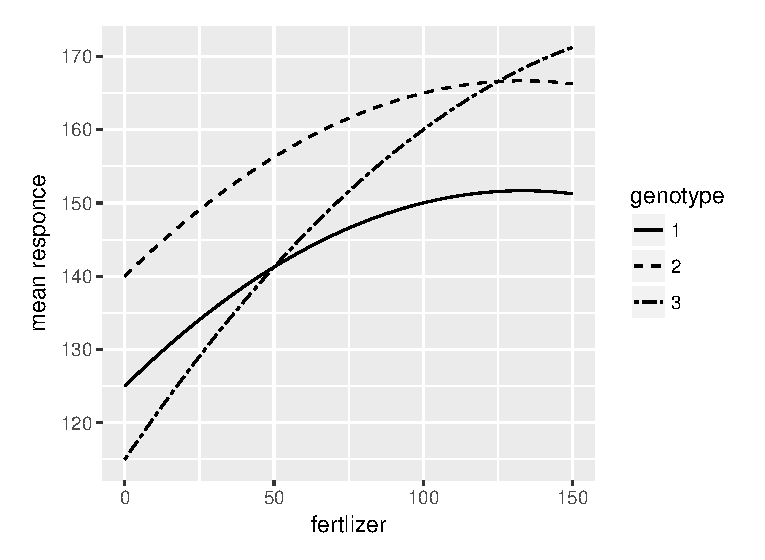
\includegraphics[width = 0.7\textwidth]{Rplot.eps}
		\end{center}

		\item 
		$\bar{y}_{11 \cdot} - \bar{y}_{12 \cdot} = -13.75,\, SE = \sqrt{\frac{\hat{\sigma}_{e}^2}{2}} = \frac{6.30128}{\sqrt{2}}$. 

		$CI = (\bar{y}_{11 \cdot} - \bar{y}_{12 \cdot} - SE \cdot t_{27, 0.975} ,\bar{y}_{11 \cdot} - \bar{y}_{12 \cdot} + SE \cdot t_{27, 0.975} ) = ( -22.8923, -4.607704)$. 
		\item 
		$\mu_{11} - \mu_{12} = -15 \in CI = (-22.8923, -4.607704)$.

		\item 
		$\bar{y}_{11} - \bar{y}_{21} = -22.5,\, SE = \frac{\sqrt{\hat{\sigma}_e^2 + \hat{\sigma}_w^2}}{\sqrt{2}} = \sqrt{\frac{39.70613 + 67.2981}{2}} =  7.314514,\, df = \frac{\left( \frac{1}{4} MS_{Block \times Geno} + \frac{3}{4} MS_{Error} \right)^2 }{\frac{1}{16} \frac{MS_{Block \times Geno}^2}{6} + \frac{9}{16} \frac{MS_{Error}^2}{27}} = 8.88$. 

		$CI = (\bar{y}_{11 \cdot} - \bar{y}_{21 \cdot} - SE \cdot t_{27, 0.975} ,\bar{y}_{11 \cdot} - \bar{y}_{12 \cdot} + SE \cdot t_{8.88, 0.975} ) = ( -39.08073, -5.919272)$.

		\item 
		$\mu_{11} - \mu_{21} = -16.25 \in CI = ( -39.08073, -5.919272)$.

		\item 
		$SE = \frac{\hat{\sigma}_b^2}{4}+\frac{\hat{\sigma}_w^2}{12} + \frac{\hat{\sigma}_e^2}{48} = \frac{MS_{Block}}{48},\, df = 4-1 = 3$. 
	\end{enumerate}
	

	\item 

	
	

	


	     
\end{enumerate}
	      

\end{document}